% !TeX spellcheck = en_US
\addscenariosection{1}{Clash Scenario}{Dragon Valley}{\images/dragon.png}

\begin{multicols*}{2}

\textbf{Author:} LAAMAKALA

\textit{A valley of secrets long forgotten. Its heart belongs to the beasts of old, while its fringes lure the bold and the desperate. Fight for power, claim the land, or perish like those before you.}

\subsection*{\MakeUppercase{Scenario Length}}
This Scenario plays out over 13 Rounds

\subsection*{\MakeUppercase{Player Setup}}
\textbf{Player Count:} 2 -- 4

\textbf{Starting Resources:} 14 \svg{gold}, 4 \svg{building_materials}, 1 \svg{valuables}

\textbf{Starting Income:} 10 \svg{gold}, 0 \svg{building_materials}, 0 \svg{valuables}

\textbf{Starting Units:}

\begin{itemize}
  \item A Few chosen \bronze\ Units
  \item A Pack of cheapest \bronze\ Units
\end{itemize}

\textbf{Town Buildings:}
\begin{itemize}
  \item \bronze\ Dwelling
  \item Each player may build the \svg{building_special_tent} building with a discount of 4 \svg{gold} and 2 \svg{building_materials}.
\end{itemize}

\subsection*{\MakeUppercase{Map Setup}}
Take the following Map Tiles ($P$ stands for the number of players) and arrange them as shown in the Scenario map layout:

\begin{itemize}
  \item P × Starting (I) Map Tile
  \item 3P × Far (II-III) Map Tiles
  \item 2P × Near (IV-V) Map Tiles
  \item P × Center (VI-VII) Map Tile (C5 is treated as a Settlement)
  \item 1 × Center (VI-VII) Map Tile with a Dragon Utopia
\end{itemize}

\textbf{Additionally, for 4 players:}
\begin{itemize}
  \item 1 × Center (VI-VII) Map Tiles with a Dragon Utopia
\end{itemize}

\subsection*{\MakeUppercase{Victory Conditions}}
The game ends at the end of the Round when any of these conditions are met:

\begin{itemize}
 \item One player has defeated each other player's Main Heroes once - \textit{That player wins the game immediately.}
 \item One player has conquered both Dragon Utopias.
 \item At the end of Round 13 (or Round 9 for a short game).
\end{itemize}

\subsection*{\MakeUppercase{Victory Points}}
If no player has achieved an immediate victory, the player with the most Victory Points (VP) wins.
In addition to the Tournament Book's ``Scoring Victory Points'' section, players get VPs for:

\begin{itemize}
 \item 5 VP for conquering a Dragon Utopia
 \item 2 VP for each enemy Main Town captured - \textit{once per captured Faction}
 \item 1 VP for every flagged Mine and Settlement on Near and Center Tiles
\end{itemize}

\subsection*{\MakeUppercase{Timed Events}}

\textbf{\nth{1} Round:}
\begin{itemize}
  \item All Heroes gain +1 \svgeven{movement}.
\end{itemize}
\textbf{\nth{4} Round:}
\begin{itemize}
  \item Remove all Black Cubes (except VII Settlement, Grail and Dragon Utopia).
\end{itemize}
\textbf{\nth{8} Round:}
\begin{itemize}
  \item Repeat event of Round 4.
\end{itemize}
\textbf{\nth{9} Round:}
\begin{itemize}
  \item Repeat event of Round 1.
\end{itemize}
\textbf{End of \nth{10} Round:}
\begin{itemize}
  \item Player(s) whose Main Hero has the least experience roll 2 \svg{resource}.
\end{itemize}

\subsection*{\MakeUppercase{Additional Rules}}
\begin{itemize}
  \item Remove ``View Earth'' from the Spell Deck.
  \item Remove ``Unexpected Reinforcements'' from the Astrologers Proclaim Deck.
  \item Split the \svg{artifact} and Spell Decks as depicted in the Tournament Book.
  \item When a Secondary Hero is recruited, that Hero gains +1 \svgeven{movement} for that Round.
  \item Trading Posts - on a single visit, trade Resources and remove Cards, OR buy a War Machine.
  \item \textbf{Sanctuary:} Gain 1 \svg{morale_positive} Token and draw a Card from your Deck. \textit{Visitable once per Faction.}
  \item \textbf{Obelisk:} Roll 1 \svg{resource} and draw a Card from your Deck. \textit{Visitable once per Faction.}
  \item When fighting a Neutral Combat, players may increase the difficulty level by +1 for an extra 5 \svg{gold} and Search (2) \svg{artifact} or \svg{spellpower}. % no-check-caps
  \item Level VII Neutral Combat cannot be skipped.
  \item If your Hero is Level VII, treat Level VI neutrals as Level VII, then gain 10 \svg{gold} for winning a Level VII Combat.
  \item A defeated Main Hero may Empower one Defense Statistic Card from his M\&M Deck and gain +1 \svgeven{movement} for the next Round.
  \item Players do not have to pay \svg{gold} after losing a Combat against another Player.
  \item When a Unit is attacked but suffers no \svg{damage-red}, it gains a Corrosion token. Remove it, when that Unit takes \svg{damage-red}.
  \item Neutral Dragons cannot be recruited in any way other than visiting a Dragon Utopia.
  \item Settlements on Center (VI-VII) Map Tiles count as two Settlements in terms of rewards AND allow rolling one \svg{resource} or \svg{treasure} (reroll any \svg{experience}).
  \item Upon visiting a Grail Field, \textbf{choose one} and then put a Black Cube:
  \begin{itemize}
    \item Receive: 10 \svg{gold}, 2 \svg{building_materials}, and 1 \svg{valuables}
    \item Search (2) \svg{spellpower} twice
    \item Search (2) \svg{artifact} twice
  \end{itemize}
  \item Dragon Utopias are guarded by 2 \azure\-tier dragons and 2 \golden\-tier dragons.
  \item Upon flagging Dragon Utopia, \textbf{choose one} and then put a Black Cube:
  \begin{itemize}
    \item Recruit one of the defeated Dragons for half its \svg{gold} (rounded down) and its \svg{valuables} cost.
    \item Receive 10 \svg{gold} AND Search (3) \svg{spellpower}.
  \end{itemize}
\end{itemize}
After visiting a Dragon Utopia, roll an Attack Die:
\begin{itemize}
  \item[\textbf{-1}] -- Dragons' Curse: The defeated Dragons’ spirits curse the land! All Heroes lose \mbox{1 \svgeven{movement}} for the next Round.
  \item[\textbf{0}] -- Dragons' Revenge: All players must sacrifice a Unit before the end of the Round; that Unit's health is reduced to 0.
  \item[ \textbf{+1}] -- Scattered Treasure: All players may lose \mbox{1 \svgeven{movement}} from a Hero next Round to Search (2) \svg{artifact} on the Map Tile that Hero is on.
\end{itemize}

\subsection*{\MakeUppercase{Suggested Houserules}}
\begin{itemize}
  \item \href{https://boardgamegeek.com/thread/3445901/custom-hex-combat-board}{Compact Battlefield}.
  \item \href{https://boardgamegeek.com/thread/3449937/houserule-for-stacking-more-than-pack}{Stacking more than Pack} - Start with Several \bronze\ Units instead of Few.
\end{itemize}

\vspace*{\fill}

\end{multicols*}

\begin{tikzpicture}[remember picture, overlay]
  \node(bg)[anchor=center, yshift=37em, opacity=0.07] at (current page.south) {
    
\includegraphics[width=1.25\paperwidth, keepaspectratio]{\art/orb_of_tempestuous_fire.png}
  };
\end{tikzpicture}
\begin{tikzpicture}[overlay]
  \centering
  \node at (4, -4) {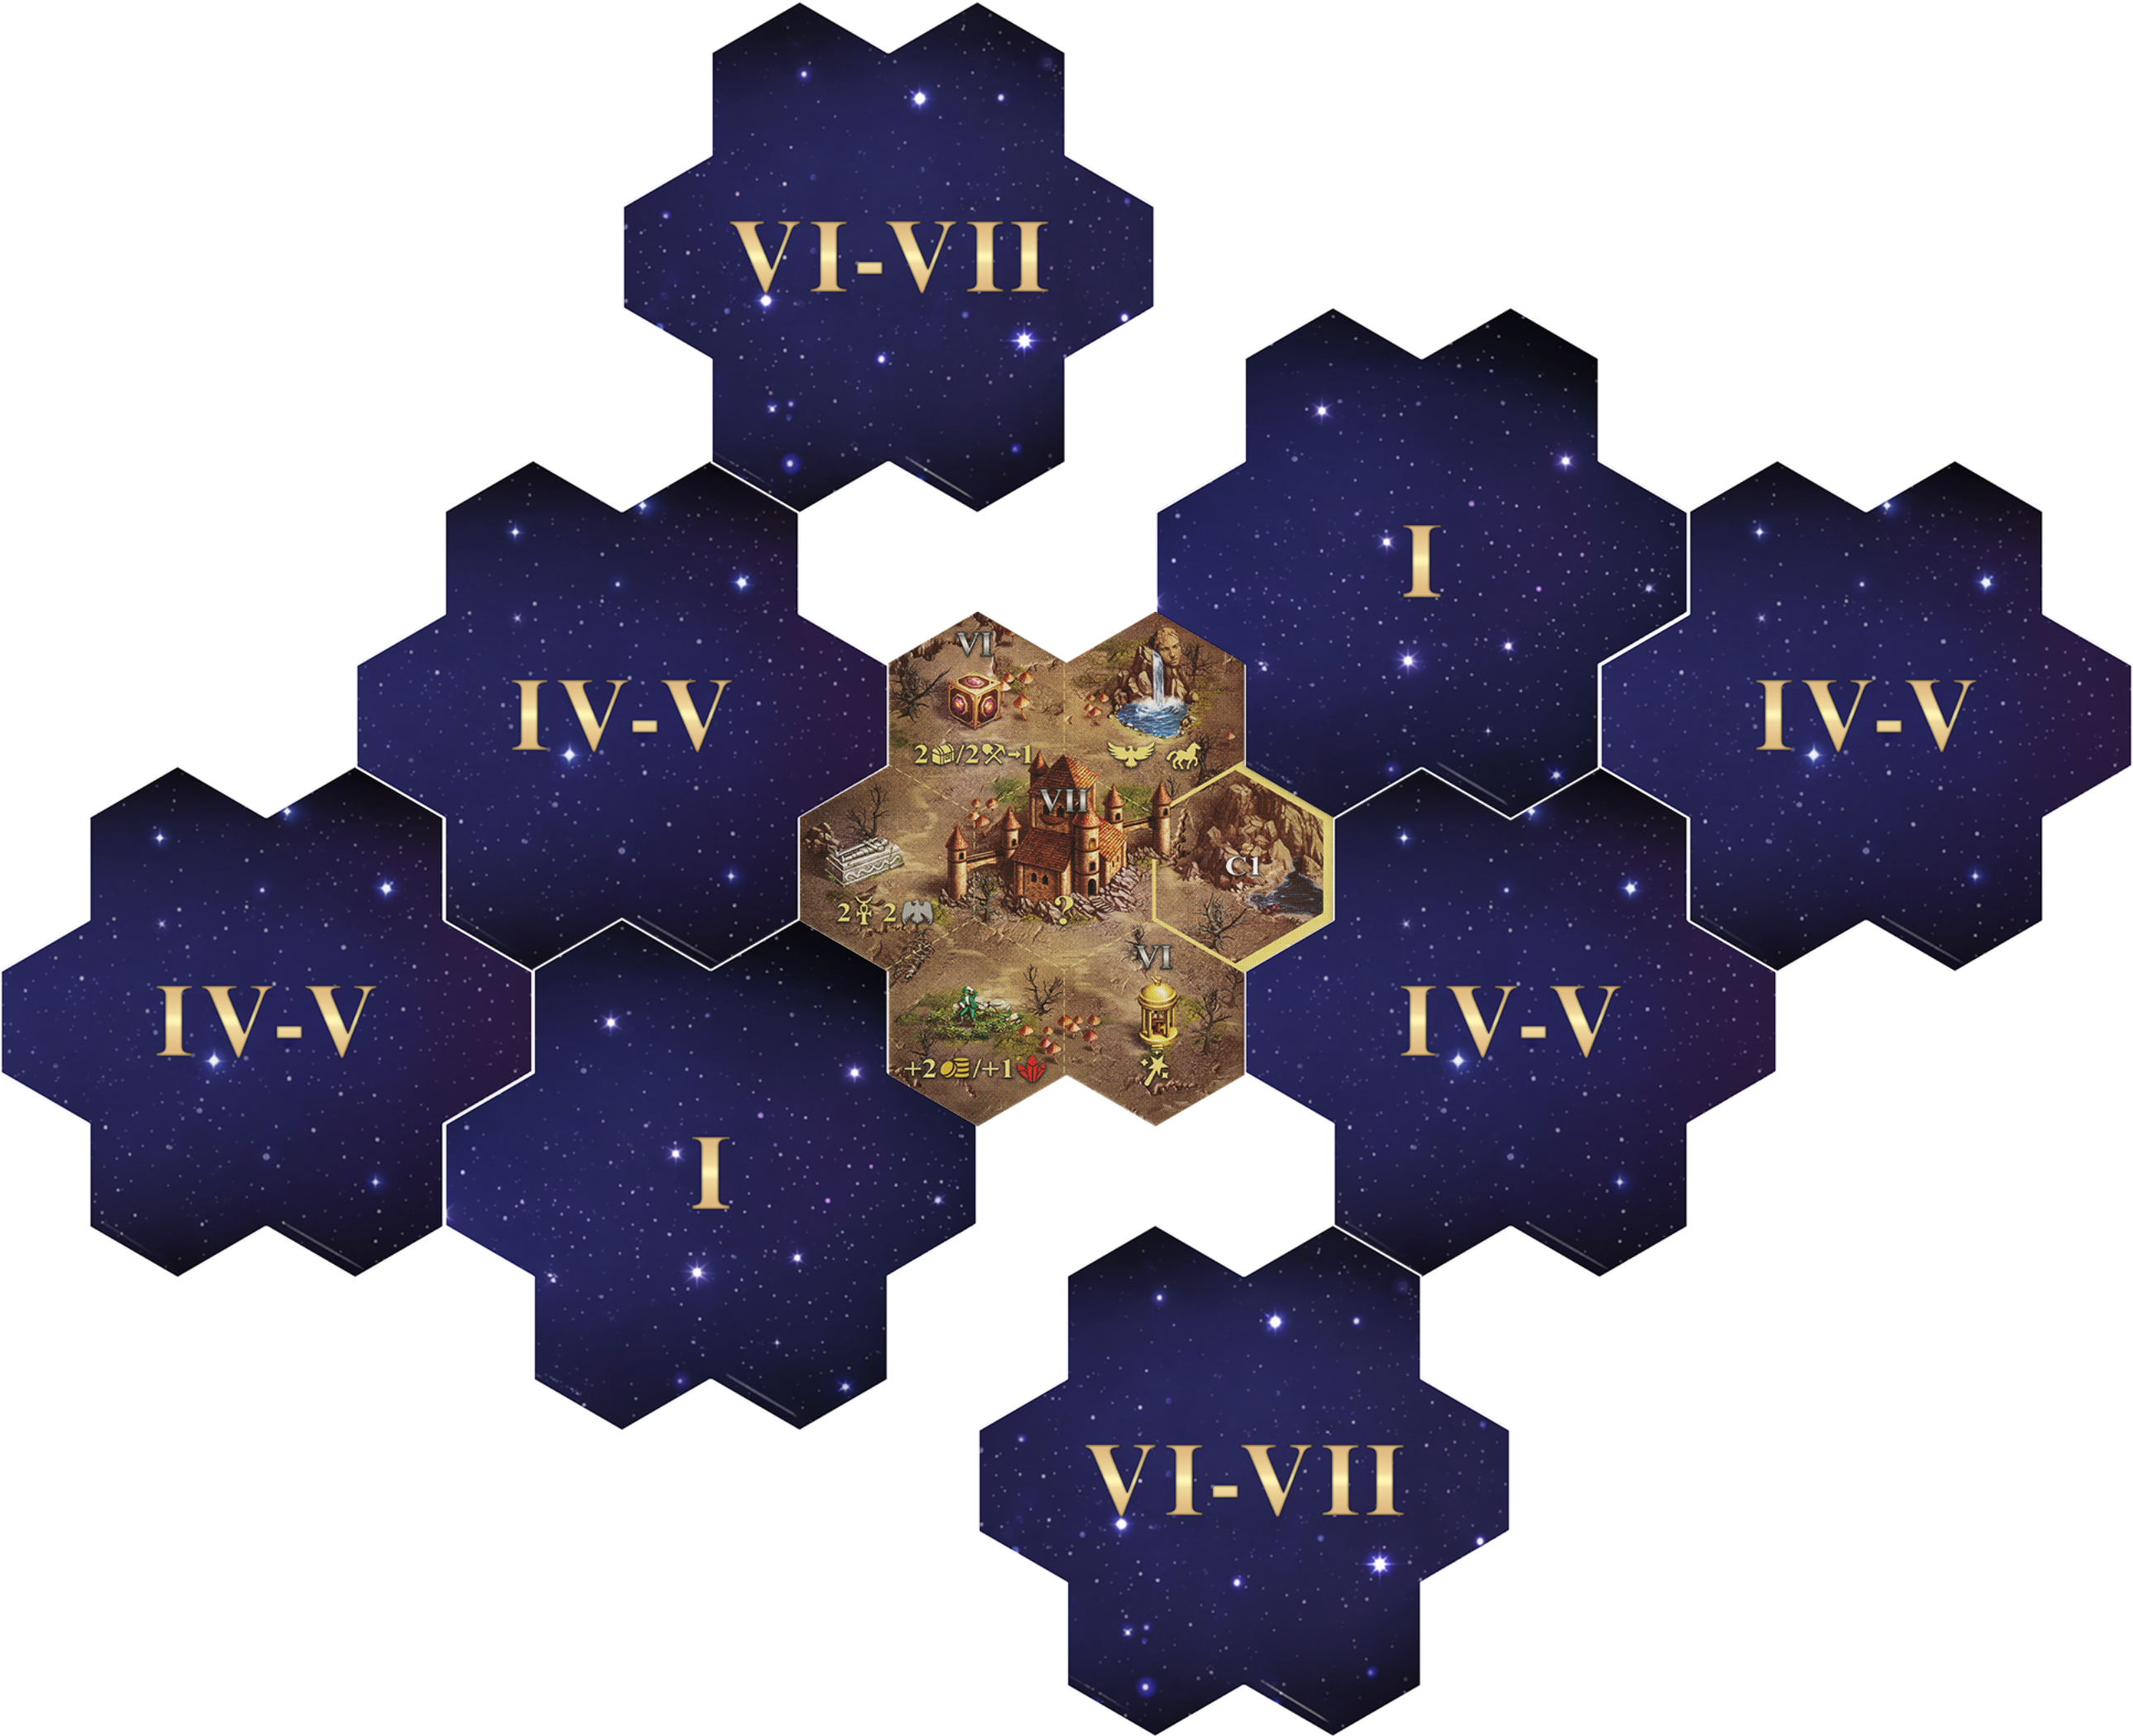
\includegraphics[scale=0.2]{\maps/dragon-valley-2p.png}};
  \node at (4, -9) {\footnotesize{\textbf{\MakeUppercase{2-PLAYER SCENARIO}}}};
  \node at (13, -4) {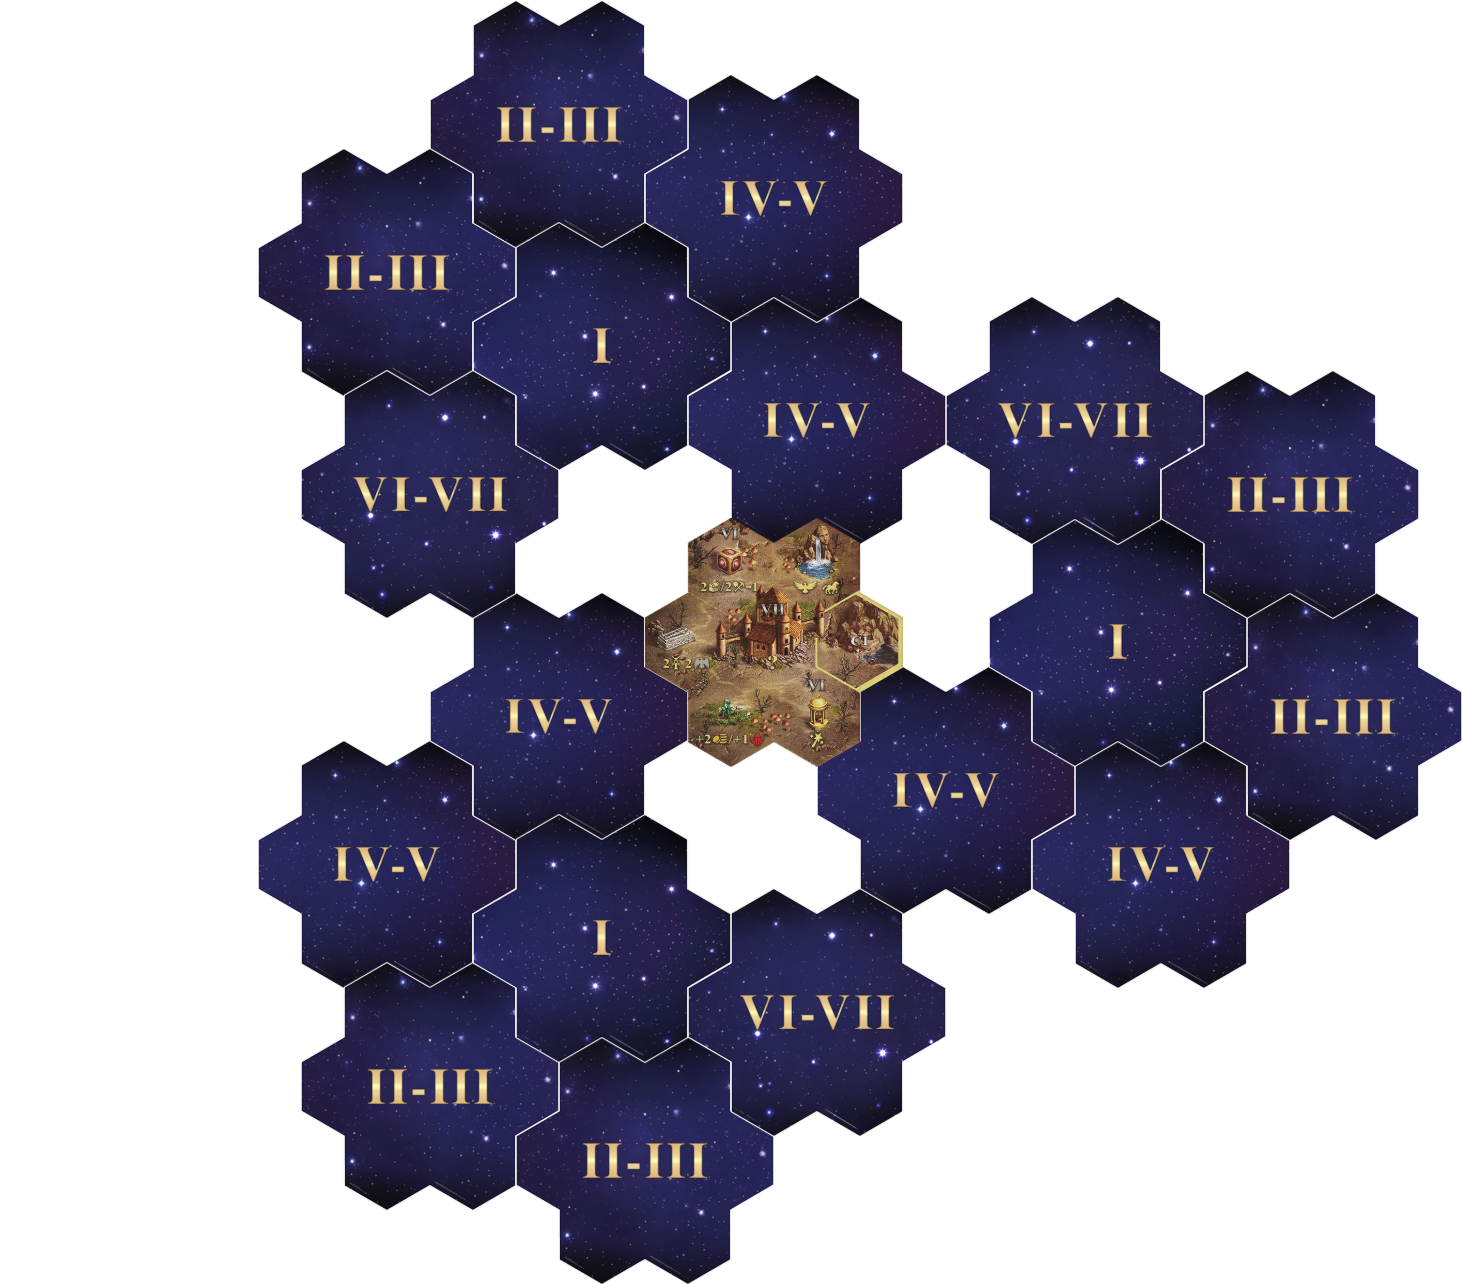
\includegraphics[scale=0.185]{\maps/dragon-valley-3p.png}};
  \node at (13, -9) {\footnotesize{\textbf{\MakeUppercase{3-PLAYER SCENARIO}}}};
  \node at (4.5, -15) {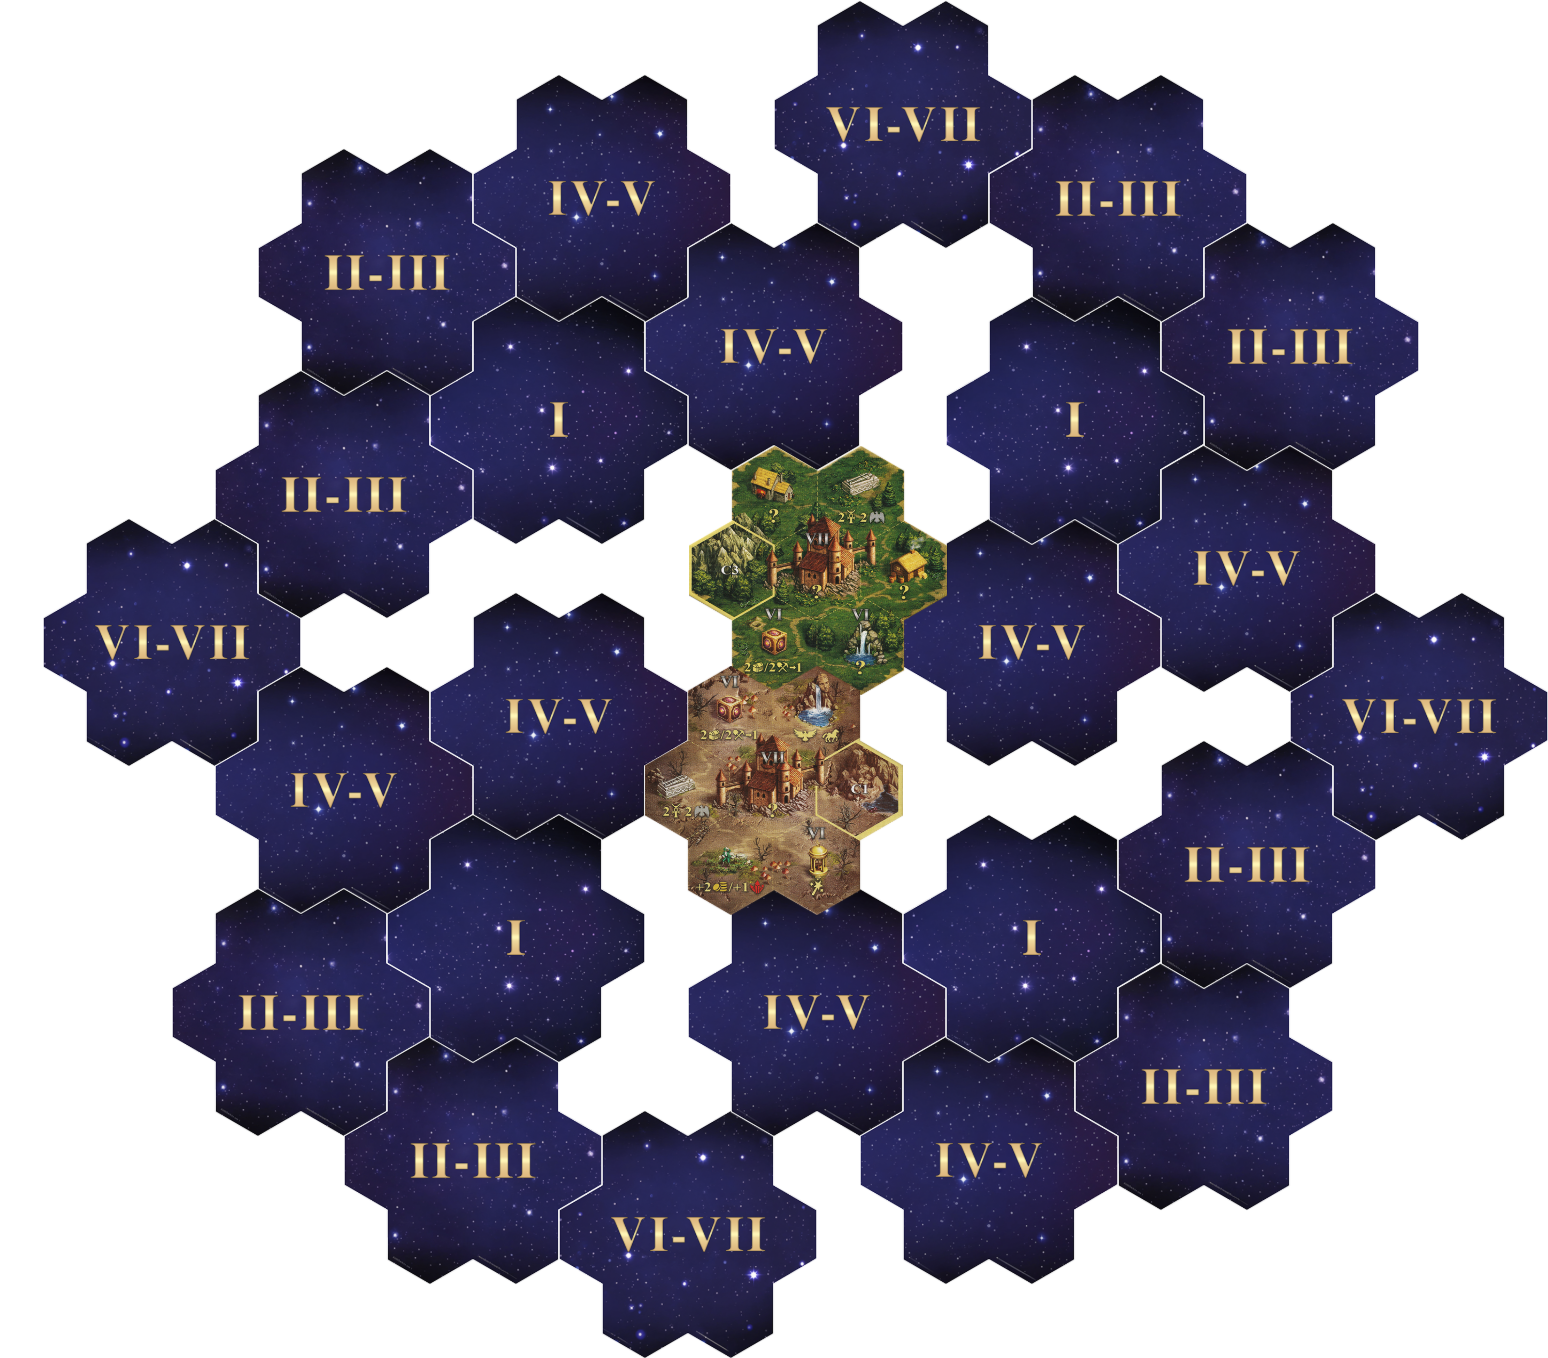
\includegraphics[scale=0.175]{\maps/dragon-valley-4p.png}};
  \node at (4.5, -20) {\footnotesize{\textbf{\MakeUppercase{4-PLAYER SCENARIO}}}};.
  \node at (14, -15) {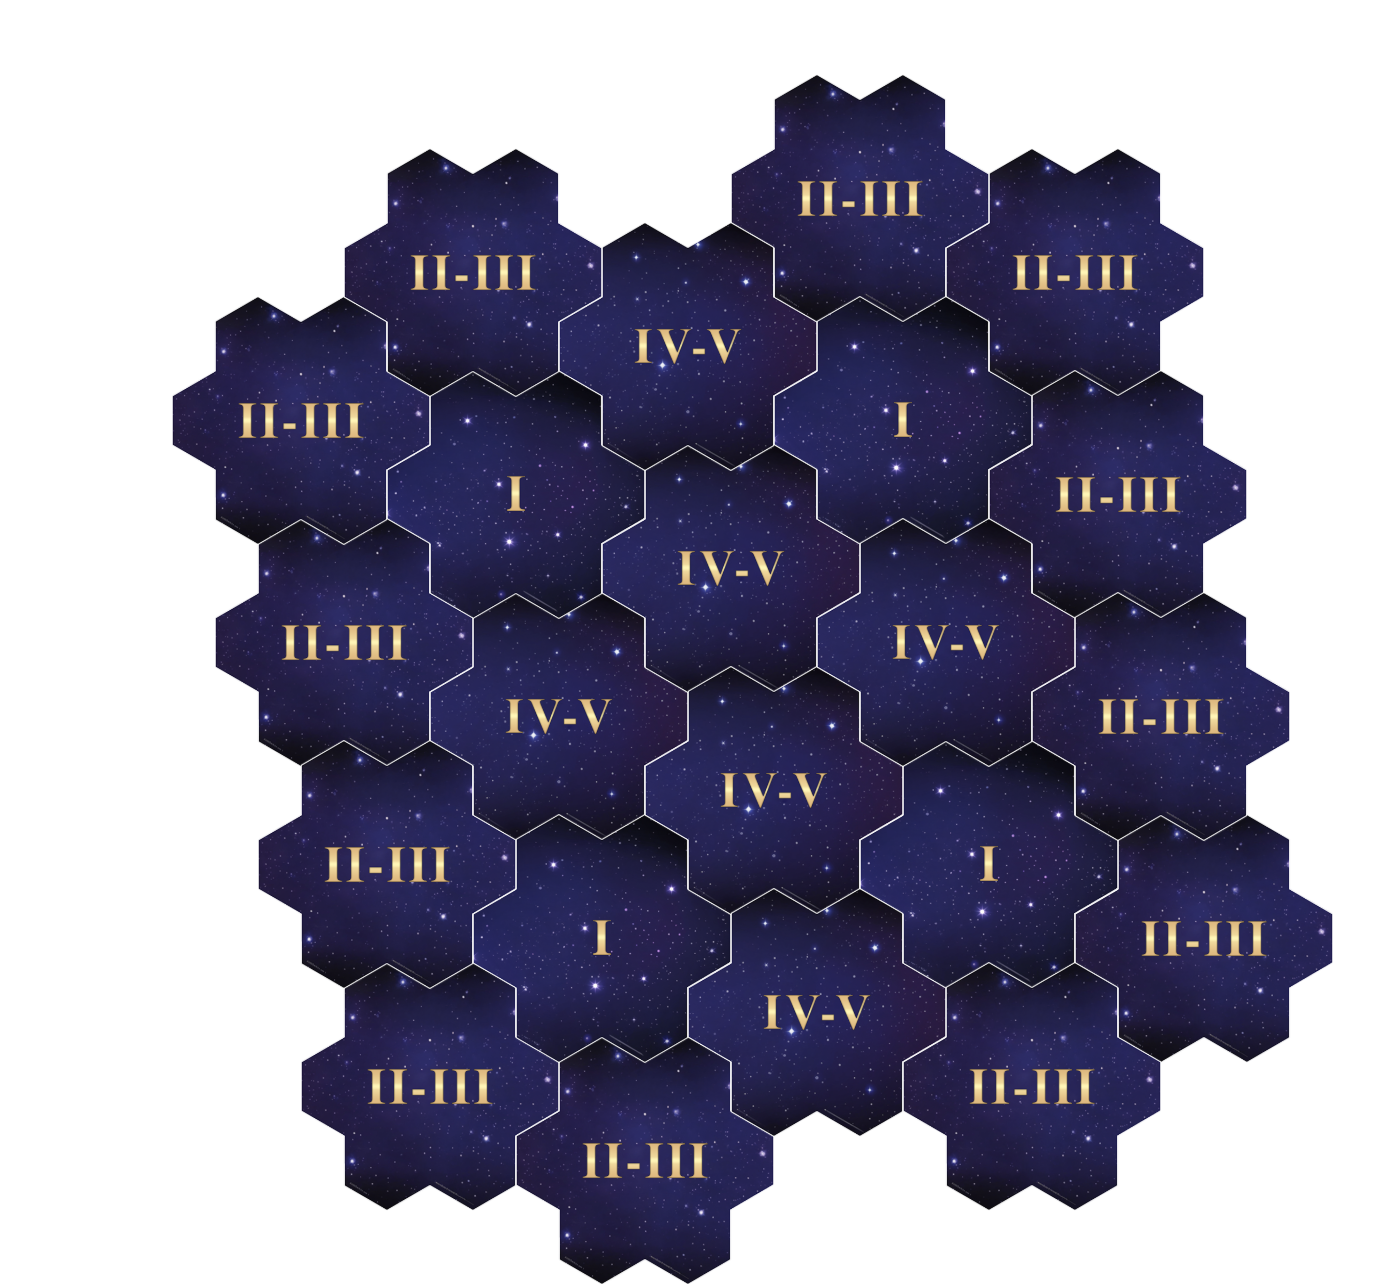
\includegraphics[scale=0.185]{\maps/dragon-valley-4p-short.png}};
  \node at (14, -20) {\footnotesize{\textbf{\MakeUppercase{4-PLAYER 9-ROUND SCENARIO}}}};
\end{tikzpicture}
